\documentclass[11pt, letterpaper]{article}
\usepackage{graphicx}
%\usepackage{natbib}
%\usepackage{vmargin}
\usepackage{subfigure, amsmath}
%\usepackage[rflt]{floatflt}
\usepackage{wasysym}
\usepackage{wrapfig}
\usepackage{url}
%\usepackage[light,first,bottomafter]{draftcopy}
\usepackage{multicol}
\usepackage{color}
\usepackage[small,compact]{titlesec}
%\usepackage[compact]{titlesec}
\usepackage{color}
\usepackage{array}
\usepackage{booktabs}
\usepackage[normalem]{ulem}
\usepackage{lipsum}

\usepackage[letterpaper,top=1.0in, left=1.0in, bottom=1.0in, right=1.0in]{geometry}

\setlength{\textfloatsep}{0.2cm} %for table spacing???


%\usepackage[letterpaper,top=1.0in, left=1.0in, bottom=.8in, right=1.0in]{geometry}


\DeclareMathOperator*{\argmax}{arg\,max}

\iffalse
\documentclass[11pt]{article}
%\usepackage[bindingoffset=0.2in,left=1in,right=1in,top=1in,bottom=1in,footskip=.25in]{geometry}
%\usepackage{blindtext}
\usepackage{graphicx}
%\usepackage{natbib}
%\usepackage{vmargin}
\usepackage{subfigure, amsmath}
%\usepackage[normalem]{ulem}
\usepackage[rflt]{floatflt}
\usepackage[square, numbers]{natbib}
\usepackage{wasysym}
\usepackage{wrapfig}
\usepackage{url}
%\usepackage[light,first,bottomafter]{draftcopy}
%\usepackage{multicol}
\usepackage{color}
\usepackage{array}
\usepackage{booktabs}
\usepackage[normalem]{ulem}

\setlength{\topmargin}{-0.75in}
\setlength{\textheight}{9.3in}
\setlength{\oddsidemargin}{-0.25in}
\setlength{\textwidth}{7.0in}
%\usepackage{fullpage}
%\usepackage[text={6.5in,8.9375in},centering]{geometry}
%\usepackage[margin=1.0in]{geometry}

%\usepackage[margin=1.0in]{geometry}
	%\addtolength{\oddsidemargin}{-.875in}
	%\addtolength{\evensidemargin}{-.875in}
	%\addtolength{\textwidth}{1.75in}

	%\addtolength{\topmargin}{-.875in}
	%\addtolength{\textheight}{1.75in}
	
%\setlength {\abovecaptionskip}{-4pt}        % Space above caption
%\newskip\subfigcapskip     \subfigcapskip    =  -4pt     %Change it to a negative number to reduce space


%\iffalse
%\setlength{\topmargin}{-0.75in}
%\setlength{\textheight}{9.3in}
%\setlength{\oddsidemargin}{-0.25in}
%\setlength{\textwidth}{7.0in}
%\fi
%\textfloatsep 11pt plus 2pt minus 4pt       % Space between main text and floats at top or bottom of page.
%\setlength {\abovecaptionskip}{-4pt}        % Space above caption
%\newskip\subfigcapskip     \subfigcapskip    =  -4pt     %Change it to a negative number to reduce space

%\usepackage{natbib}
%\bibliographystyle{apalike}
\fi

\bibliographystyle{IIE}

\newenvironment{packed_itemize}{
\begin{itemize}
  \setlength{\itemsep}{1pt}
  \setlength{\parskip}{0pt}
  \setlength{\parsep}{0pt}
}{\end{itemize}}

\newenvironment{packed_enumerate}{
\begin{enumerate}
  \setlength{\itemsep}{1pt}
  \setlength{\parskip}{0pt}
  \setlength{\parsep}{0pt}
}{\end{enumerate}}

\newenvironment{packed_description}{
\begin{description}
  \setlength{\itemsep}{1pt}
  \setlength{\parskip}{0pt}
  \setlength{\parsep}{0pt}
}{\end{description}}

\newtheorem{theorem}{Theorem}
\newtheorem{definition}{Definition}
\newtheorem{question}{Question}
\newtheorem{lemma}{Lemma}
\newtheorem{observation}{Observation}
\newtheorem{gap}{Research Gap}


%% Tighest margins for NSF
%\setpapersize{USletter}
 %\setmarginsrb{1in}{1in}{1in}{1in}{0in}{0in}{0in}{0in}
 %\setmargrb{0.9in}{0.2in}{0.9in}{0.5in}
 %\def\spacingset#1{\renewcommand{\baselinestretch}{#1}\small\normalsize}
 %\def\spacingset#1{\renewcommand{\baselinestretch}{#1}\small\normalsize}
 %\pagestyle{plain}
 
\begin{document}

\setlength\intextsep{0pt}

\begin{center}
	\huge
	{\bf Recommender systems with capacity } 
\end{center}

\begin{center}
	\large
	{\bf Final Project Report \\				
		Computational Social Processes CSCI-4110/6110 }
\end{center}	 

\begin{center}
	\large	 
	Seyed Shahab Mofidi\\
	Anders Maraviglia\\
	Fall 2016
\end{center}

%add abstract?

\section{Introduction}
Let us start by a familiar example most readers can relate to. As a host, I prepared food for a group of friends whom I invited to my house. Since a few of my guests were vegetarian, I had to prepare two dishes; veggie option and non-veggie with some forecasts of how many of my guests are omnivore and how many are not. As usual, a margin of error was considered in my prediction and two dishes were prepared. On the night of the event, my omnivore guests were interested in the veggie dish more and ate the food they were not supposed to, let my vegetarian guests leave with empty plates. Many what if scenarios struck my mind after that event. But the main question was how to design a better mechanism that ensures a better outcome.

Through this example, we illustrate a central mechanism (the host) who recommends a set of available alternatives (dish(es)) to multiple agents (guests). Undoubtedly, this example is a simplified version of what organizations, firms and companies deal with as a decision making problem to understand how to design a recommendation system that guarantee systematic performance while their members, users, and customers preferences are also considered. In fact, the problem of our interest in this paper, applies to environments that share five fundamental characteristics which we highlight here. \textbf{(1) \emph{Hierarchical decision making process}}. The problem of our interest is similar to leader-follower game models in terms of the decision makers roles in which the leader (i.e., host in this case) should decide and move first (i.e., prepare dishes) with some perceptions of the follower(s) (i.e., agents) reactions. After the leader makes decisions, the agents decide and move afterwards (i.e., what to eat). Moreover, the leader has no control on the agents choice. (i.e., the host cannot force guests what to eat). \textbf{(2) \emph{Limited available resources}}. When infinite amount of a resource is available, recommendations by the system is only centered on the preferences of each agent isolatedly since even if all agents' first choice is alternative "a" for example, all can obtain their first choice. However, when a resource is relatively scarce to the number of agents interested, challenges arise as who should take priority among agents, and what are the associated costs to the system as the consequences. Study these challenges and consequences is to our interest. 
In the dinner party example, imagine if more food had been prepared, the outcome would not have been the same. However, it comes at a higher price of sacrificing host's budget for an ordinary dinner or a larger amount of food leftovers. \textbf{(3) \emph{Simultaneous personalized recommendations}}. Agents receive recommendations either all at the same time (simultaneous) or in an order (sequential) through a time horizon. In sequential recommendations, system recommends to each agent one at a time. The set system recommends to a new agent can be updated based on the choice(s) of the previous agent. Hence, the recommendation's context depends on the place of the agent in the queue. And so the problem boils down to what should the order of the queue be (imagine the host make a line at the dinner table and put vegetarian guests first) which is out of scope of this work and readers are encouraged to read [cite]. 
In simultaneous recommendations, system's decision-making process happens once and agents' choices come afterwards. The simultaneous recommendation set(s) to agents are often aggregate in the system. (i.e., single recommendation available for group(s) of agents). [or have zero overlaps]. E.g., one food table for all guests at the dinner party).
We are interested in the simultaneous \emph{personalized} recommendations problem which is very complicated specifically when resources are finite. Because
in this case, the system needs to incorporate all agents' preferences in advance and thus need more accurate information about the agents choice. 
In the above example, the problem could have been solved if the food is served to each guest individually, however, guests should have filled a questionnaire in advance to provide information on their diet, preferences, food allergies, etc.  \textbf{(4) \emph{Myopic independent rational agents}}. When you are at the table as a guest, your choice of food only depends on your personal preference and almost nobody considers how his/her choice can affect others as it was the case in this example, and what the omnivore guests did. However, the overall outcome could be improved if the system intervenes with it's holistic view. Here, limiting the omnivores choice to the non-veggie option (i.e. not offering them to the vegetarian dish) would be a proper example of system's intervention.
Therefore, when agents are myopic independent rational individuals, the personalized recommendation set can be used as an intervention tool for the system to guarantee the achievement of some major concerns.
\textbf{(5)\emph{Two objectives are not necessarily aligned}}. In these types of problems, leader's objective is to maximize benefit (minimize costs) while agents are utility maximizers and sometimes these two objectives do not agree. Here in this example, omnivore guests who ate veggie dish maximized their own utility while the host's objective was to satisfy all of his guests.  

Underlying many applications in recommendation systems are these five characteristics. One of the emerging application is the ``\emph{sharing economy}''  with market valued at \$75 billion \cite{allen2015sharing}. The sharing economy is where resources owned by independent entities are collectively shared through a central mechanism with internet-based platforms who owns no resources; instead operates a marketplace (e.g., companies like Uber, Airbnb, TaskRabbit, etc.). Critical to a central mechanism's success is its ability (1) to entice large participation by agents and (2) to accommodate their preferences to ensure repeat participation. Agents expect high-quality service (e.g., tasks completed to desired specifications within a given time). This is achieved when the central mechanism takes a systematic view of allocating  limited resources to agents.  Agents benefit from a large pool of alternatives and when the central mechanism retains some control to ensure service expectations are met.  Agents desire autonomy and discretion to decide when and how they want to provide access to their resources  based on their individual preferences. If discretion is not provided, this limits agent participation.  Thus, success in sharing economy depends on agents satisfaction.  However, agents preferences are not always aligned with system objectives. Take for example a ride-sharing application, like Uber or Lyft.  The agents are drivers that prefer riders with destinations on their current route or to a high populated area (where another rider is likely). The central mechanism wants to maximize the number of successful matches by assigning the closest driver to a rider.   

Another application is in the retail industry where, a company like Macy's  wants to offer it's customers a personalized set of in-store coupons of limited inventory through emails. These coupons are tailored based on limited leftover %(excess)
inventory of some retail locations or regional clearances. Therefore, there are couple of products here and there that Macy's wants to offer to specific customers at a lower price. 
Crucial to maximize revenue is Macy's ability to offer the right set(s) of coupons to the right group(s) of customers such that no customer receive excessive list of in-store coupons which are not to her interest (guarantee her return to the store) and are not available in near-by locations (guarantee her satisfaction). Again worth noting that the inventory is limited and the challenge is limiting some customers to receive all coupons since Macy's cannot guarantee to satisfy all demand. Moreover, customers also have the discretion not to buy any products and hence, at the same time incentives exist for Macy's to offer same coupons to a larger group of customers. 

One more application is in the emerging electric car industry, mobile application companies (e.g., PlugShare) recommend charging station alternatives to electric car users. However, the number of charging stations are limited and the charging process is not as fast as pumping your car at a gas station yet and each car occupies stations for a long period of time. PlugShare should also take the congestion factor of stations as well as your convenience preference of the nearest and fastest service into consideration when making recommendations.

We also presented our research project through the course project assignment motivation where each group has to choose a project topic from a list of different topics available by the instructor. All projects are available to all groups in the class. No group can choose more than one topic and two groups can not work on the same project. Moreover, the instructor has preferences over the assignments (i.e., which topic is done by which group) due to particular skills needed for a specific project. For example, one project is a software development project where a special programming language is needed that only few groups are able to deploy. Difficulties arise when a topic is left unselected (i.e., rejected by all groups) and some topics are selected by two or more groups (i.e., duplicates occur). Therefore, the instructor has to intervene and adjust the assignments considering the ability of groups as well as their preferences.

In all fo these examples, all of the five mentioned characteristics are present. Therefore, this research is interested in determining the \textit{optimal personalized assortment} to recommend to each agent in these environments. By optimality, we mean maximum systems benefit with regards to the decision behavior of rational utility maximizer agents. In deed, the agents' decisions create dependencies in the system that impact system benefit when limited resources are available. We describe two common approaches that currently exist for the central mechanism design of  recommender systems which can be considered as two extreme cases for the spectrum which we study. \textbf{(1)\emph{Centralized}}, and \textbf{(2)\emph{Decentralized}} approaches. 

In the centralized approach, system is the only decision maker and the agents follow orders without any discretion. System performance is the only objective, the choices are dictated to the agents, and their preferences are not taken into account (i.e., either ignored by the system or their preferences are not available to the system). An example of this approach is the well-known Vehicle Routing Problem (VRP). In VRP, fleet dispatcher (central mechanism) matches the optimal set of destinations and corresponding routes to a fleet of vehicles in order to meet the demand of certain nodes with optimal systematic performance (e.g., minimum cost). In environments where agents are committed to the system and are employed by the company, the only objective is to improve the performance of the system, and the agents either do not have any preferences or their preferences are not taken into consideration in the solution space of the system. 
Moreover, the central decision making assures the solution to be optimal, no resource constraint is violated, double efforts and underutilization is minimized (i.e., two agents do not visit single node and empty travels are at the minimum possible). The decision making in the centralized approach often needs to be fast. In addition, achieving the optimal solution depends on the full compliance of the agents which is not a false assumption in this case. Another example would be the job assignment problem where tasks are optimally assigned to machines for different time spans. Obviously machines have neither preferences over the jobs nor the ability to disobey the assigned jobs.

On the other end of this spectrum is the decentralized approach where agents are the only decision-making individuals with personal preferences. All alternatives are available to all agents who make selections based on their own preferences, and the system does not limit agent's options.  
A decentralized approach applies in environments where social welfare (i.e., sum of all agents' utilities) of the agent's are at the top priorities (e.g., customer satisfaction). This is due to the fact that agents often have no commitments to the system and hence, no dictatorship applies here. The central mechanism usually facilitates agents' decision making process through  personalized recommendations which are very well-known as recommender systems (e.g., Google, Netflix, etc.). If you are searching for a hotel to spend two nights of your vacation in, of course Google can not force you to pick a choice but can navigate you through a list of endless choices. These types of recommender systems employ machine learning techniques (i.e., collaborative and content-based filtering are two extremely popular methods and interested readers are referred to[cite]) to presume agents preferences and increase agents participation to improve the chance of matching an agent with an alternative. In a decentralized approach, systematic performance is ignored, and high utilization is compromised due to multiple agents' common interests in some alternatives lead to other alternatives left unselected. Therefore, decentralized control can result in reduced systematic performance \cite{roughgarden2005selfish}. For example, decreasing the number of unoccupied room of a hotel, visitor's travel distances, city congestions are not a concern in Google recommender systems. Moreover, number of alternatives recommended are hypothetically infinite and decision making process for agents receives more effort compared to when the central mechanism makes decisions. Table \ref{spectrum}) summarizes the advantages and disadvantages of these two approaches.

Neither of these two extreme approaches are applicable when the five mentioned characteristics exist in a recommendation system because neither are able to fully harness underutilized resources. For example, in a centralized approach, Uber's central mechanism takes a rider-centric view by recommending a single rider's alternative to the closest driver (ignoring driver's destination preferences).  The driver has 15 seconds to either accept or reject the recommended alternative.  Uber has policies to strongly encourage high driver acceptance rates. Uber's current centralized approach limits who can participate as a driver  because drivers must be committed to Uber tasks.  If drivers want to interleave a ride-share with their planned travels, they cannot because the central mechanism does not take into account driver preferences when recommending rides. In a centralized approach with limited discretion, agents preferences are not taken into account. Hence, it affects systematic performance negatively. Also, decentralize approach will not fit the Macy's example. All coupons cannot be offered to all customers. By the time they come to the store, the deal might not be available at that store, or some other customer might already have bought the specific product and either the customer leave the store dissatisfied or Macy's has to reduce the price of a substitute product which Macy's had not intended to do so. The reader can easily verify why a centralized is not applicable here.
Also, for the charging station example, PlugShare  company takes decentralized approach and shows the specification (e.g., locations, number of stations, charging adaptors, etc.) of all nearby stations to all drivers and lets them choose. Although it also shows customers the data on the number occupied slots, it does not have any control on drivers choice. For example if only one slot is available and two cars pick the same stations as their destination, one of them would be dissatisfied and has to either wait or pick another further station which adds to the inefficiency of the system. If the system recommended some other alternatives, higher utilization could be achieved. A smarter and more efficient way is to consider the user's preferences (e.g., the car type, convenient locations, etc.) as well as the overall systematic performance (e.g., demand of a particular station, congestion, other users preferences, etc.) when making recommendations. 
 
Therefore, a new approach is needed to combine the advantages of a centralized approach (e.g., less participant effort, quicker time to match, systematic resource allocation) with the advantages of a decentralized approach (e.g., agent discretion and privacy, increased participation opportunities). We study a hybrid approach that provide agents with an assortment of limited personalized recommendations. This hybrid mechanism is a  hierarchical approach in which the central mechanism considers agents' preferences, as well as systematic performance and interdependencies, when creating personalized recommendations. First, the central mechanism makes personalized recommendations consisting of a set of alternatives to multiple distributed independent agents.  Then, agents have discretion to make selections or rejections based on their own unique valuation of the recommended set. Observed system outcomes are a function of what is recommended and decentralized selections. This approach enables holistic resource allocation and can enforce service level requirements. Also, agents retain autonomy and discretion. Personalized recommendations eliminates the need to evaluate a large numbers of  alternatives, reduce the effort required from participants, and thus, can increase agents satisfaction. Our model facilitates this type of central mechanism design, and incorporates  holistic allocation of decentralized agents' discretion opportunities into a systematic optimization framework.  

\begin{centering}
	\begin{table}[hbt]
		\caption{\emph{Central Mechanism Approaches}} \label{spectrum}
		\small
		\begin{center}
			\vspace{-.2in}
			\noindent \resizebox{1.0\textwidth}{!}{
				\begin{tabular}{p{0.22\linewidth}p{0.23\linewidth}p{0.24\linewidth}p{0.31\linewidth}}
					\hline
					 & \textbf{Centralized \newline Approach}  & \textbf{Decentralized \newline Approach} & \textbf{Our Hybrid \newline Approach} \\
					\hline
					System's  \newline Performance          & Considered          & Not Considered  &  Considered \\ 
					\hline
					Agents' \newline Preferences          & Not Considered          & Considered & Considered\\   
					\hline
					System          & Dictatorship & No Intervention & Partially Intervenes \\ 
					\hline
					Agents      & Committed 
					& No Commitment  & No Commitment \\ 
					\hline
					Decision Making \newline Process & Fast and Efficient & Takes Time and Effort & Moderate\\ 		
					\hline
					Common Examples        & \textbf{Assignment \newline Problem}
					& \textbf{Recommender \newline Systems}  & \textbf{Bilevel \newline Optimization} \\ 
					\hline
			\end{tabular}}
		\end{center}
	\end{table}
\end{centering}  

In this research, we advocate for a more flexible recommendation scheme that is neither fully centralized nor decentralized; yet minimize participant effort, enable a quick time to match, and facilitate systematic resource allocation. It must also privilege agent discretion and privacy, and it should increase participation opportunities. We study the role of the central mechanism as a moderator who makes personalized recommendations of limited resources to agents. 

In order to do so, we model the problem as a bilevel optimization problem where the system moves first and agents pick their choices based on what systems offers. We explore different solution methods and heuristics to achieve higher performances in terms of solution time. However, the outcomes of the heuristics are slightly different. Then we compare our results with the well-known gale shapely algorithm.


\section{Related literature} \label {lit}
\subsection{Matching problem} 
Matching problems are a well-studied area with numerous applications. Although the differed acceptance algorithm (Gale and Shapely, 1962) [cite] is the footstone of this work, different problems have different criteria and axiomatic properties (e.g., pareto optimality, stability, strategy proofness, social welfare). And it is not a one-fit all scenario.  So, other solution methods (e.g., serial dictatorship, top trading cycles, etc.) have emerged with unique properties that address the needs of those specific problems. 

While stability in the matching problem has attracted lots of attentions, few works also consider other aspects of the matching problem. For example, Anshelevich  [cite] argues that a stable match might not necessarily be a socially desirable outcome. It is backed up by the fact that stable matching problem only considers the ranking of agents and thus social welfare is not guaranteed to be optimal. In another work, Kadama and Kojima  slightly modified the definition of the stability under existence of the distributional constraints (i.e., regional caps). One of the application of their model is allocation of medical match market of doctors and hospitals when the government enforces certain distributional constraints to overcome geographical imbalance. Although their main goal is still the stability, they allow certain blocking pairs to remain in what so called stable match because otherwise it may violate the caps. This is very similar to our work because the capacity constraints are imposed by a central system (global entity or enterprise). However this central system does not have any control over the choices of agents and thus no recommendation has been made to agents. Also this central system has no incentive to match certain agents. 

\subsection{Sharing economy}
Existing sharing economy descriptive studies include qualitative studies 
\cite{bardhi2012access, belk2014you, corciolani2014gift, deakin2010markets,  johnson1998growth, lewis2012p2p, murphy2016shared}, and econometric models  \cite{cullen2014outsourcing, fradkin2015bias}.   

Prescriptive mathematical models to guide decisions in sharing economy is a new area of research.    In \cite{jiang2016collaborative}, pricing and quality decisions are decided for a monopolist manufacturer's physical resource that can be used by its primary owner or made available via a sharing economy. In \cite{benjaafar2015peer}, an equilibrium model is developed for a two-sided  market in which agents may not be able to find a alternative (and vice versa).    Both consider a decentralized approach. An emerging area of sharing economy research is dynamic ride-sharing, which matches drivers with riders to share one-time trips  \cite{agatz2012optimization,  furuhata2013ridesharing, kleiner2011mechanism, li2014share, stiglic2016making, winter2006ad, xing2009smize} and peer-to-peer car sharing \cite{hampshire2011peer, hampshiresinhasimulation,   shaheen2013carsharing, steininger2014extending}; all consider either a fully centralized or fully decentralized approach.

Multiple agents with discretion capabilities concerning recommendations from a central mechanism are unstudied.  Related is \cite{wang2014stable}, in which  systematic  and agent preferences are considered by enforcing dynamic ride-sharing matches to be stable.  Also, in \cite{powell2000value} a central mechanism recommends a single alternative to a single dispatcher who can accept or reject it.     %A single dispatcher's 
The acceptance probability is represented by an exogenous random variable.  Neither incorporate discretion into the optimization model, capture the entire spectrum of discretion levels, nor  consider dependencies in systematic performance due to multiple agents' decisions.  

\subsection{Recommender systems}
Vast literature on how to create personalized recommendations exists.  However, recommender systems research assumes what is being recommended has an infinite capacity, and does not consider users' selections interdependencies  \cite{adomavicius2005toward, amatriain2011data, condliff1999bayesian, ekstrand2011collaborative, lops2011content, pazzani2007content, schafer2007collaborative}. For example, personalized recommendations of articles to read, movies to stream, or ads to click all can be simultaneously consumed without impacting systematic performance.     
By contrast, this research seeks to  create personalized recommendations to multiple decentralized users whose simultaneous selections impact systematic performance. 

\subsection{Bilevel optimization}
The central mechanism must consider agents' likely selection behavior when making the personalized recommendations, because agents have discretion not to comply with the recommendations they do not prefer.  Also, agents' selection is highly influenced by the recommendation. Thus, bi-level programming will be used.      
Bi-level programming problems, also known as Stackelberg leader-follower games \cite{bracken1973mathematical, von1952theory}, model a hierarchy in which a leader makes decisions that effect the followers' feasible decision set \cite{bracken1973mathematical,  candler1977multi, colson2007overview}. Bi-level optimization problems are recognized as difficult \cite{dempe2016solution}; even linear bi-level programming is NP-hard \cite{audet1997links, bard1998practical, frangioni1995new}. Generalized bi-level optimization approaches in which the followers' decision variables  are discrete  remains computationally challenging \cite{moore1990mixed, xu2012three, zeng2014solving}.  

Bi-level research has mainly focused on developing specialized algorithms for specific problems.  Prominent bi-level optimization problems include transportation network design, network interdiction, assortment optimization, and revenue management. The network interdiction problem models the attacker-defender problem and specialized approaches (e.g., decomposition approaches and step inequalities) have been shown effective in solving many different variants of this problem \cite{delgadillo2010analysis, lim2007algorithms, scaparra2008bilevel, sullivan2014convex}. In transportation network design problems, the network design and its capacities are leader decisions; followers solve shortest path problems \cite{brotcorne2001bilevel, farahani2013review, gao2005solution,  marcotte1986network}. Assortment optimization determines what product assortment to offer to an aggregated set of shoppers, who then make consumer selection choices from the recommended assortment \cite{kok2015assortment}. In all problem types, a single aggregate leader decision is made and shared among the followers.   For example, all users make routing or interdiction decisions using the same shared network, and all consumers make purchasing selections from the same product assortment.  Capacity constraints of a single shared assortment have been considered in assortment optimization \cite{feldman2015capacity, gallego2014constrained, rusmevichientong2010dynamic}.     
Revenue management research considers what assortment of products (e.g., flight tickets) to display to what segment of users at varying times to sell remaining capacity of a finite resource \cite{gallego2014general, kunnumkal2010new,   zhang2009approximate, zhang2005revenue}.  Existing revenue management work assumes demand selections occur sequentially and recommendations are independent of each other. Similarly, dynamic assortment optimization considers personalized recommendations of finite capacities to sequentially arriving customers \cite{bernstein2015dynamic, johari2016know, saure2013optimal, topaloglu2013joint}. In contrast, this work makes multiple, \emph{simultaneous} personalized recommendations of finite capacity alternatives. 


Existing work in bi-level optimization either models the leader problem as deciding (i) a single aggregate recommendation, or (ii) multiple independent recommendations. The bi-level models proposed in this research are innovative because the leader problem has to make multiple personalized recommendations of finite capacity alternatives.  Specialized solution approaches are required because the personalized recommendations  cannot be made independently, as systematic performance is dependent on multiple agents' selection outcomes.     

\section{Model} 
The bilevel optimization framework consists of a central mechanism as a leader  and agents as followers. The central mechanism leads by deciding what personalized set of alternatives to recommend to multiple decentralized independent agents.  The agents' utility-maximizing selection processes follow from the personalized recommendations. 
The model considers two disjoint sets: $j \in S$, the set of agents (which have discretion capabilities), and $i \in R$, the set of alternatives, where $R=D\cup N$. The set $D$ consists of alternatives; the set $N$ consists of the no-choice selections, and $D\cap N=\emptyset$.   The recommendations are made simultaneously to all agents and a single period model is presented. Alternatives are assumed to have a capacity of 1. Other notations are as follows.

   
\vspace{-.1in}
\begin{flushleft}
{\bf Decision Variables:}
\end{flushleft}
\vspace{-0.1in}
\begin{tabular}{l@{\quad}l}
$x_{ij}$ & 1 if the central mechanism recommends alternative $i\in R$ to agent $j \in S$; 0 o.w. \\ %(leader variable)
$y_{ij}$ & 1 if agent $j \in S$ selects alternative $i \in R$; 0 o.w. \\ %(follower variable)\\
%$o_{ij}$ & 1 if alternative $i \in R$ is selected by a single supply user $j \in S$ (1-to-1 match); 0 o.w. \\
$z_{i}$ & 1 if more than one agent selects alternative $i \in D$ (duplicate); 0 o.w.  \\ %(leader variable) \\
$w_{i}$ & 1 if no agents select alternative $i \in D$ (full rejection); 0 o.w. \\%(leader variable) \\
\end{tabular}
\vspace{-.1in}

\begin{flushleft}
{\bf Parameters:}
\end{flushleft}
\vspace{-0.1in}
\begin{tabular}{l@{\quad}l}
$C_{ij}$ & Systematic benefit of recommending alternative $i \in R$ to agent $j \in S$. \\
%$p_{ij}^{l}$ & Probability that alternative $i$ is selected by supply user $j$, given discretion level $l$ \\ 
$u_{ij}$ & Agent $j \in S$ utility of alternative $i \in R$. \\ %, given discretion level $l$ \\
$a_i$ & Maximum number of agents  recommended alternative $i\in R$, \\ & %given discretion level $l$ 
 where $a_i = |S|$ if $i \in N$, and $1 \leq a_i \leq |S|$ if $i \in R$. \\
$b_j$ & Number of  alternatives (including no-choice) recommended to agent $j \in S$. \\ %& given discretion level $l$ ($0 \leq b_j^l \leq |D|$)\\
$m_j$ & Number of  alternatives (including no-choice) agent $j \in S$ can select. \\ %& given discretion level $l$ \\
%$f_i$ & Number of supply users that can fulfill alternative $i$ \\
$d_i$ & Duplication penalty if alternative $i \in D$ receives  more than one  selection. \\
$r_i$ & Full rejection penalty if alternative $i \in D$ is not selected by all agents. \\ 
%$l_d$ & Lower limit on the recommended matches that include alternative $d$ \\
%$l_s$ & Lower limit on the recommended matches to supply slot $s$ \\
\end{tabular} 
%}
\vspace{0.1in}





%\vspace{-0.45in}

\begin{flushleft}
\textbf{Bi-Level Optimization Formulation: }
\end{flushleft}
%\vspace{-.1in}
\begin{align}
 \max			& \displaystyle\sum_{i \in	R} \displaystyle\sum_{j \in S}  C_{ij} y_{ij} - \displaystyle\sum_{i \in D} d_i	z_{i}	- \displaystyle\sum_{i \in D} r_i w_{i}		\label{systemobjective} \\
    s.t.       & \displaystyle\sum_{j \in S} x_{ij} \leq a_i  \quad\forall i \in R \label{upperdemand}\\
&\displaystyle\sum_{i \in R} x_{ij} \leq b_j   \quad\forall j \in S \label{uppersupply}\\
& \displaystyle\sum_{j \in S} y_{ij} \leq |D| z_{i} + 1   \quad\forall i \in D \label{duplicateconstraint} \\ 
& 1-\displaystyle\sum_{j \in S} y_{ij} \leq w_{i}  \quad\forall i \in D \label{fullrejectionconstraint} \\ 
&  x_{ij} \in \{ 0,1 \}  \quad \forall i \in R, j\in S  \label{variables_leader2} \\
&  z_{i} \in \{ 0,1 \}; w_{i} \in \{ 0,1 \}  \quad \forall i \in D \label{variables_leader1} \\
& \max \displaystyle\sum_{i \in	R} \displaystyle\sum_{j \in S} u_{ij} y_{ij} \label{followerobjective} \\
& 	s.t. \quad y_{ij} \leq x_{ij}  \quad\quad\forall i \in R, j \in S \label{hookingconstraint} \\
& \quad \quad \displaystyle\sum_{i \in	R} y_{ij} = m_j  \quad\forall j \in S \label{upperlevelofselection}\\ 
&  \quad \quad  y_{ij}  \in \{ 0,1 \} \quad  \forall i \in R, j\in S \label{variables_follower}		
\end{align}

%\vspace{-.2in}
For a better grasp on the bilevel formulation of this problem, one can consider the network representation of alternatives and agents in figure \ref{fig:network}, where the system maximizes the flow from node $s$ to node $t$ in the upper level problem. Maximizing flows backwards from node $t$ to node $s$ are the lower level problem.
\begin{wrapfigure}{R}{0.46\textwidth}
	\centering
	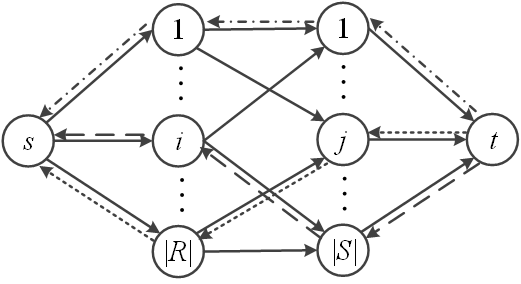
\includegraphics[width=0.51\textwidth]{network_rep.png}
	\caption{\emph{Example of the network structure. Solid arcs: leader's established arcs (centralized system recommendations), Dotted arcs: followers' final flow (supply users choices)}}   \label{fig:network}
\end{wrapfigure}  
\noindent

The central mechanism's leader problem is captured in (\ref{systemobjective})-(\ref{variables_leader1}).
The objective function (\ref{systemobjective}) is to maximize the expected systematic benefit by recommending sets of alternatives to multiple agents.  It captures the dependencies among agents' selections by accounting for penalties of duplicate and fully rejected alternatives, which are a function of the agents' decisions (followers).  
Constraints (\ref{upperdemand}) enforce at most $a_i$ agents can be recommended alternative $i \in D$.  Constraints (\ref{uppersupply}) enforce $b_j$  alternatives (including no-choice) are recommended to agent $j$.  Constraints  (\ref{duplicateconstraint}) and (\ref{fullrejectionconstraint}) capture the dependency among multiple agents, whether a alternative is selected by more than one agent (duplicate); or whether a alternative is not selected by any agents (full rejection), respectively.   


The agents' follower problems are captured in (\ref{followerobjective})-(\ref{variables_follower}). The agents are rational decision makers who make selections based on maximizing their own perceived utility of alternatives in the personalized recommendations (\ref{followerobjective}), selecting the top $m_j$ alternatives in descending order ranked on $u_{ij}$ values. Constraints (\ref{hookingconstraint}) enforce their selections to be a subset of system's recommendation. 
In this model, no-choice set $N \in R$ represents discretion in which agents do not have to select all alternatives.   
The leader and the followers decisions variables are binary in constraints (\ref{variables_leader2})-(\ref{variables_leader1}), and (\ref{variables_follower}) , respectively. 

\subsection{Solution method}
The proposed bi-level framework is a discrete linear bilevel programming problem (DL-BLPP) [cite Bard book, page 240] and can be solved with off the shelf solver. [put MATLAB function]. However, the solution time is increasing exponentially and thus become intractable for large scale problems. See figure\ref{fig:runtime1}.
\begin{wrapfigure}{R}{0.46\textwidth}
	\centering
	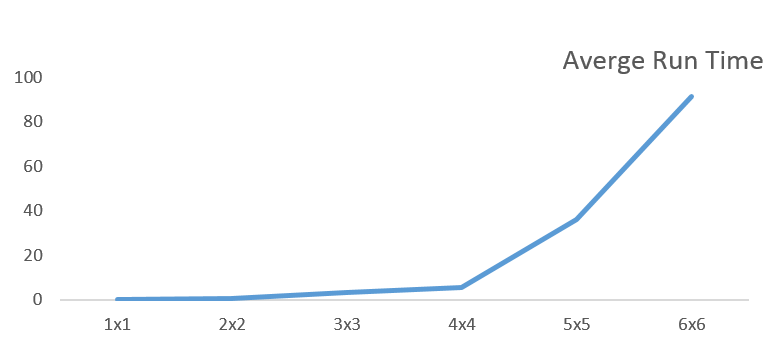
\includegraphics[width=0.47\textwidth]{runtime_pic.png}
	\caption{\emph{DL-BLPP}}   \label{fig:runtime1}
\end{wrapfigure}  
\noindent

Due to integer values for $m_j$, the lower level problem is unimodular and hence the integrality for lower level variables can be relaxed to continuous. (i.e., constraints (\ref{variables_follower}) are relaxed to $0\leq y_{ij} \leq 1$). This makes the problem to be a discrete-continuous linear  bilevel programing problem (DCL-BLPP) which is slightly easier to solve Although algorithms exists to deal with these types of problems [cite Bard book, page 240]. But challenge in solving large scale problems remains the same.

The outcome of this optimization is two matrices: a recommendation matrix $X$ and a agent selection matrix $Y$. It worth noting that multiple optimal solutions exits.

\subsection{Heuristic 1, projection method}
 One way of capturing this alignment in the model is employ the projection method that projects the agents' $j$'s utility vector $\vec{U}_{j}$ onto the systematic benefit vector $\vec{C}_{j}$ associated with each agent $j$. Therefore, a projection matrix $P$ captures the alignment of $U$ on $C$ by the well known projection function in (\ref{projection}). 

\begin{wrapfigure}{R}{0.46\textwidth}
\centering
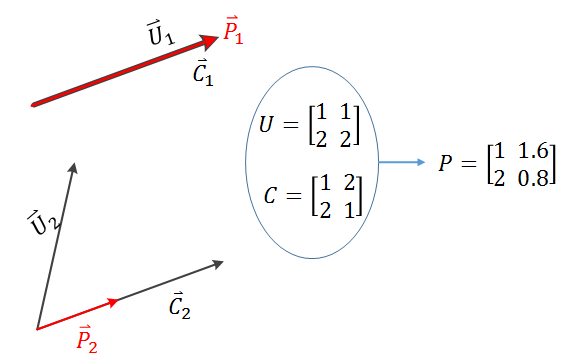
\includegraphics[width=0.47\textwidth]{projection_example.png}
\caption{\emph{Example of two vectors}}   \label{fig:projection}
\end{wrapfigure}  
\noindent
\vspace{-.1in}
\begin{align}
\vec{P}_{j}=Proj_{_{\vec{C}_{j}}}\vec{U}_{j}=\frac{\vec{U}_{j}.\vec{C}_{j}}{||\vec{C}_{j}||^2} \vec{C}_{j} \label{projection} 
\end{align}

Figure \ref{fig:projection} illustrates an example of this alignment concept where $\vec{C}_{1}$ and $\vec{U}_{1}$ are completely aligned to each other whereas $\vec{C}_{2}$  and $\vec{U}_{U}$  are not. The projection matrix $P$ represents a compact information of $U$ and $C$ together where the magnitude by which the vector $\vec{U}_{j}$ is aligned to vector $\vec{C}_{j}$

\begin{flushleft}
	\textbf{ Single Level Optimization Formulation: }
\end{flushleft}
Applying this technique, we are able to combine both levels into one single level optimization as shown below.
\begin{align}
\max			& \displaystyle\sum_{i \in	R} \displaystyle\sum_{j \in S}  P_{ij} y_{ij} - \displaystyle\sum_{i \in D} d_i	z_{i}	- \displaystyle\sum_{i \in D} r_i w_{i}		\label{singleobjetive} \\
s.t.       & \displaystyle\sum_{j \in S} x_{ij} \leq a_i  \quad\forall i \in R \label{upperdemandproj}\\
&\displaystyle\sum_{i \in R} x_{ij} \leq b_j   \quad\forall j \in S \label{uppersupplyproj}\\
& \displaystyle\sum_{j \in S} y_{ij} \leq |D| z_{i} + 1   \quad\forall i \in D \label{duplicateconstraintproj} \\ 
& 1-\displaystyle\sum_{j \in S} y_{ij} \leq w_{i}  \quad\forall i \in D \label{fullrejectionconstraintproj} \\ 
& 	 y_{ij} \leq x_{ij}  \quad\quad\forall i \in R, j \in S \label{hookingconstraintproj} \\
&  \displaystyle\sum_{i \in	R} y_{ij} = m_j  \quad\forall j \in S \label{upperlevelofselectionproj}\\ 
&  x_{ij} \in \{ 0,1 \}; y_{ij}  \in \{ 0,1 \}  \quad \forall i \in R, j\in S  \label{vars} \\
&  z_{i} \in \{ 0,1 \}; w_{i} \in \{ 0,1 \}  \quad \forall i \in D \label{variables_leaderproj} 
%& &  &  y_{ij}  \in \{ 0,1 \} \quad  \forall i \in R, j\in S \label{variables_follower}	
\end{align}

\noindent

The single level formulation is similar to the bilevel formulation except that in the single level formulation, the follower objective function (\ref{followerobjective}) is not present. Also, the upper level objective function in the bilevel formulation (\ref{systemobjective}) is replaced with the objective function (\ref{singleobjetive}) which maximizes the benefit by applying the projection method (\ref{projection}) and yet captures the dependencies among agents' selections by accounting for penalties of duplicate and fully rejected alternatives. All other constraints remain the same as before and are presented in a single level.


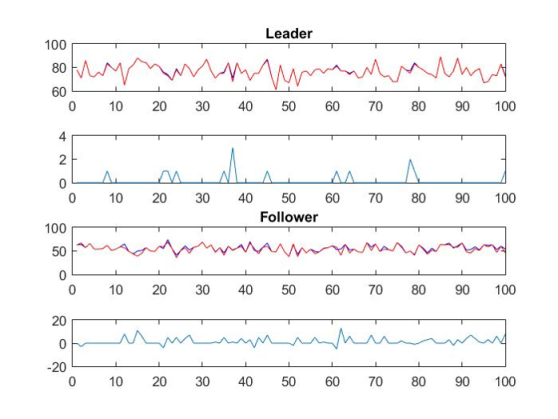
\includegraphics[]{comparison.png}
\\
\caption{\emph{Bilevel performance vs single level performance. Charts from top to bottom: (1) leader's bilevel objective function in dark blue, leader's single level objective funtion in red. (2) difference between single and bilevel optimizagtion. (3) followers's bilevel objective function in dark blue, leader's single level objective funtion in red. (4) the difference between the two. }}   
\label{fig:comparision}
\noindent

The proposed single level framework is a mixed integer programming (MIP) and numerous algorithms and solvers exist that solves the MIP very efficiently in reasonable time. We used branch and bound technique to solve this in MATLAB [cite code used]. Experiments of different sizes have been tested and the results are compared to the results of the bilevel optimization. A comparison of hundred iterations of recommendations of 5 alternatives to 5 agents is shown in the figure (\ref{fig:comparision}) where the $U$ and the $C$ matrices are randomly generated. However, as illustrated in the figure, the leader's objective function of the single level optimization is near optimal. Moreover, inconsistencies occur for the follower's objective function in single level solution (i.e., some times lower and some times higher). Therefore, we study other heuristics and compare the performances. 

\section{Heuristic 2, greedy method}
We also tested an alternative to the bilevel optimization framework, which attempted to reconcile deferred acceptance algorithms like Gale Shapley [add citation] with the greedy algorithm paradigm in order to maximize system performance at the sacrifice of social welfare utility.  It should be noted that in doing so the stable matching requirements held as being a central property in deferred acceptance algorithms are not a concern for ours.  Also note that the susceptibility of our greedy algorithm to manipulation was not evaluated, in order to focus efforts on examining the algorithms potential viability.  

In order to evaluate the greedy algorithms effectiveness, we decided to use the Gale Shapley algorithm as a baseline and compare its system performance and social welfare to that of our algorithm.  However, we had to adapt Gale Shapley to accommodate for many to many matching. 

\subsection{Greedy Algorithm for Many to Many Matching}
The user matrix represents the preferences of the agents being proposed to.  The system matrix represents the preferences of the agents doing the proposing.  Proposal order is determined by taking the sum of the utilities for each column in the user matrix, where this is basically determining individual system desirability for all users, and from this a list of systems is created, sorted by desirability in decending order.  We then iterate over this list, and each system then picks their highest rated (available) users, up to the maximum allowed matches.  

Note that each system and user can have at most the maximum allowed matches at any given time, but each system and user does not necessarily have a complete matching at the end of the algorithm.  This case is more thoroughly examined in the Gale Shapley algorithm discussion.   

	\subsection{Example}

\subsection{Gale Shapley Algorithm Adaptation for Many to Many Matching}
At it's core, this is a standard implementation of the Gale Shapley algorithm, which basically ensures a stable one to one matching between two agent sets.  The difference here is that we allow many to many matching.  Many to many matching is done by allowing each proposer to make at most max matches proposals each iteration.  An important case to mention is when a proposer tried to match to a proposee with the max matches and tie breaking needs to happen.  This is done by taking the old proposer with the lowest utility beaten by the new proposer out of the proposee match list and adding them back to the match queue.  This, combined with the rest of the Gale Shapley algorithm, means the possibility exists that a full many to many matching for any two input matrices does not necessarily exist.

	\subsection{Example}

\subsection{Experiment Results}

%\subsection{insights}
%1- How much misalignment is ok to still get the same solution out of both methods	

\section{Conclusion and future steps}
This research studies the case where system performance is a major concern when matches are assigned. However, this does not come at the price of ignoring agent's preferences in recommendations. So, the recommendations are made to agents considering their preferences under the priority of system's performance. Comparing the results of our greedy algorithm to DA stable matching algorithm, we conclude that the system performance in our greedy approach is more than or equal to DA stable matching and the social welfare in our greedy approach is less than or equal to the DA stable marching algorithm. 
For future works, we want to calculate the bound on this comparison and measure the maximum possible difference in system performance as well as social welfare in both algorithms. In order to do so, we need to consider worse case scenarios. 
Moreover, in this study, we set the alternatives to propose first to guarantee optimality for the system. However, to fully harness the characteristics of this problem, agent-proposing method still needs to be studied as well. 
\iffalse
\begin{flushleft}
	{\bf high level notes:}
\end{flushleft}
\vspace{-.1in}
1- Central mechanism = social planner, match maker, recommender system (maybe)

\noindent
2- Other motivations = Macy’s coupons, governmental distribution constraints, recommending nearest charging station for electrical vehicles

\noindent
3- customized Assortment planing = menu design, incorporate customer choice behavior into revenue management

\noindent
4- Shape customer demand

\fi


\newpage
%\bibliographystyle{IIE}
\setcounter{page}{1}
\bibliography{CAREER2014}
\end{document}


\iffalse
\section{More on sharing economy}
``Access becomes more valuable than ownership in the future'' as Bostman predicts in her book [cite]. The things we own, have extremely low utilization rates and spend most of their useful lives idle \cite{botsman2011s}. Consequently, our day-to-day lives are full of many underutilized resources. The next time you are at a stoplight, count the empty seats in vehicles around you. Open a closet in your house, and try to remember the last time your power drill or camping tent was used.  Consider the  duplication of effort when both you and your neighbor make individual grocery trips. A more efficient use of resources would be to ride together. Society is demanding greater utilization of limited resources.  In essence, by promoting access over ownership, a novel way to achieve a resource-efficient future is through the increased utilization of underutilized resource capacities. Peer-to-Peer Resource Sharing Systems [P2PRSS] are where resources owned by independent entities are collectively shared through a central mechanism. The shared resource can be a physical resource (like a power drill) or a human resource (like the ability to perform a task). P2PRSS are part of the sharing economy and collaborative consumption movements \cite{botsman2011s}. Media coverage has been plentiful, including \emph{Time Magazine} naming sharing as one of the ``10 ideas that will change the world,'' \cite{TimesSharing}, as well as featured articles in \emph{The Economist} \cite{EconomistSharing}, [INSERT others].      
Peer-to-peer sharing exists for spare rooms (Airbnb), rides (Uber, Lyft), tools (Sharehammer), warehouse space (FLEXE), cars (RelayRides), Flightcar, designer clothes (ReFashioner), gardens (campinmygarden),talents (TaskRabbit, Freelancer), commercial spaces (DesksNearMe), training (Skillshare), companionship (Match.com), community activities () 
and much more.  Non-profit groups like the American Logistics Aid Network (ALAN) match logistics capabilities with the needs of communities and relief agencies in response to a disaster. Projects like TeamUp facilitate the matching of volunteers to run errands with cancer patients. Capital investment into these Systems in the past few years has been significant with the sharing economy being valued at \$26 billion  \cite{botsman2011s}.    
The P2PRSS market is valued at \$75 billion \cite{allen2015sharing} with investments made by start-up and Fortune 500 companies,  not-for-profits,  and government entities \cite{EconomistSharing} with the largest investment of \$2 billion since 2012 being invested by start-ups  [citation].  
Success of P2PRSS companies (e.g., on New Year's Eve more than a million people slept in a locale's extra space found on Airbnb rather than a hotel \cite{AirbnbNYE}), (e.g., each night 40,000 people sleep in a locale's extra space found via Airbnb rather than a hotel \cite{EconomistSharing}), (since 2008 over 11 million visitors have been matched with locals' extra spaces) and TaskRabbit (over XXXX tasks have been completed by individual freelancers), 
illustrate their disruptive potential to make significant changes to the way we consume products and services. P2PRSS represent an emerging concept that has the potential to have significant economic, environmental, and social benefits in the US (CITE articles and papers). In 2013, the US Conference of Mayors passed the Shareable Cities Resolution, pledging that mayors will resolve to make their cities more shareable and to establish task forces to review and address regulations in their municipalities that may hinder participation.  

P2PRSS use internet-based platforms to provide wide-reach visibility into untapped resource capacity.  This has the potential to increase resource visibility, utilization, accessibility, and flexibility.  Thus,  if designed and operated with societal goals in mind, P2PRSS have the potential to be powerful social, economic, and environmental forces transforming how businesses operate and people live. However, P2PRSS are inherently more complex than traditional systems because they rely on a crowd of independent entities (denoted as Supply Owners) to provide access to their resources. Agents are the primary owners of the resources and get to decide whether or not to allow access to their resources.   Alternatives are indicated needs for resources made by secondary users who do not own the resources.  A Central Mechanism is a third-party organization responsible for managing the interactions between the agents and the alternatives.  The central mechanism owns no resources; instead operates a marketplace.  

Critical to a central mechanism's success is its ability  (1) to entice large participation by both agents and alternatives and (2) to accommodate their preferences to ensure repeat participation. Alternatives expect high-quality service (e.g., tasks completed to desired specifications within a given time). This is achieved when the central mechanism takes a systematic view of allocating agents' distributed resources.  Alternatives %shouldnt it be agents?
benefit from a large participation pool of agents and when the central mechanism retains some control to ensure service expectations are met.  Agents desire autonomy and discretion to decide when and how they want to provide access to their resources  based on their individual preferences. If discretion is not provided, this limits agent participation.  Thus, capacity % better to say availbility or inventory
in P2PRSS depends on agents satisfaction.  However P2PRSS participant preferences are not always aligned. Take for example a ride-sharing application, like Uber or Lyft.  The agents are drivers that prefer riders with destinations on their current route or to a high populated area (where another alternative is likely).  Riders want to be picked up quickly (preferring the closest driver).  The central mechanism wants to maximize the number of successful matches and repeat participation by both agents and alternatives.

Existing P2PRSS central mechanism design takes either a centralized or a decentralized approach.  A centralized approach provides limited discretion options for agents. This enables the central mechanism to make matches quickly and with minimal effort from participants.  However, this limits agent participation because no autonomy is provided to choose alternatives fitting their current routines. For example, Uber's central mechanism takes a rider-centric view by recommending a single rider's alternative to the closest driver (ignoring driver's destination preferences).  The driver has 15 seconds to either accept or reject the recommended alternative.  Uber has policies to strongly encourage high driver acceptance rates. Uber's current centralized approach limits who can participate as a driver  because drivers must be committed to Uber tasks.  If drivers want to interleave a ride-share with their planned travels, they cannot because the central mechanism does not take into account driver preferences when recommending rides. In a centralized approach with limited discretion, agents preferences are not taken into account. %systematic performance is negatively impacted because of high rejection rates and/or low participation. % and with limited discretion opportunities results in Uber drivers being dedicated drivers (although the system does allow flexibility for when a agent wants to access the system).       %deactivated agent accounts if the acceptance rates is too low.  %and in training tells them should accept 80 percent of all the ride alternatives they receive, but "the closer to 100 percent the better." %The number of rejections  which they can say yes or no to rides  and the number of rejections is limited.  the option to  and 
%Uber tells drivers that they should accept 80 percent of all the ride alternatives they receive, but "the closer to 100 percent the better." Business Insider Article
%The other category is a fully decentralized system when all alternatives are provided to all agents.  
The other current design is a decentralized approach in which agents make selections based on their own preferences when all alternatives are made available (e.g., Airbnb, FLEXE).  Because agents have a myopic view  or do not have the time to evaluate all possible alternatives available, decentralized control can result in reduced systematic performance \cite{roughgarden2005selfish}.   In a decentralized system, systematic performance is not considered, and it is common for some alternatives to receive multiple selections (duplicate) and others to receive none (full rejection) 
\cite{VergeTaskRabbit}. A decentralized approach also requires time and effort to be exerted by agents to find and evaluate suitable matches, which increases the time to match and decreases agent participation rates. For example, taskers have complained about the time required to find jobs in Taskrabbit, where on average, taskers spent two hours a week looking at open tasks for matches in a decentralized system \cite{VergeTaskRabbit}. For these reasons neither current approaches to central mechanism design are able to effectively harness underutilized resources. 

A new approach combining the advantages of a centralized approach (e.g., less participant effort, quicker time to match, systematic resource allocation) with the advantages of a decentralized approach (e.g., agent discretion and privacy, increased participation opportunities) is to have the central mechanism facilitate interactions between agents and alternatives through  personalized recommendations. %better to say customized assortment
A hierarchical approach in which the central mechanism considers agents' preferences, as well as systematic performance and interdependencies, when creating personalized recommendations is needed.
First, the central mechanism makes personalized recommendations consisting of a set of alternatives to multiple distributed agents.  Then, the agents have discretion to make selections or rejections based on their own unique valuation of the recommended alternatives. Observed system outcomes are a function of what is recommended and decentralized selections. This approach enables holistic resource allocation and can enforce service level requirements. 
Also, agents retain autonomy and discretion. Personalized recommendations eliminates the need to evaluate a large numbers of  alternatives, reduce the effort required from participants, and thus, can increase agent satisfaction. Our model facilitates this type of central mechanism design, and incorporate  holistic allocation of decentralized agents' resources requires discretion opportunities into a systematic optimization framework.  
[research questions should be added here]
\fi	



Here, the central mechanism only has partial information about $u_{ij}$ values.  %agent's utilities.  
\uline{Discrete choice models will capture %that both exogenous and endogenous factors that influence user selection.  In a consumer choice model, 
	agent selection probability as a function of the composition of the personalized recommendation and   %Selection probabilities are conditioned given as distributions over all possible recommendation sets.  %permutations of alternative sets.  
	that a agent's selection changes based on what alternatives they have been recommended.}   % and users may accept a substitute alternative if their most preferred is not recommended. 
Random Utility Models (RUMs) \cite{train2009discrete} are a type of discrete choice model in which individuals select the recommended alternative with the maximum utility; and utility is only partially observable to the central mechanism. Utility in RUMs is decomposed into two parts linearly as: $u_{ij}=V_{ij} + \epsilon_{ij}$, where $V_{ij}$ is the observable utility, %(also known as representative utility)
and $\epsilon_{ij}$ is the random utility.    Depending on the choice model, different assumptions are made about the distribution of the random utility.  


The follower problems given in (\ref{followerobjective})-(\ref{variables_follower}) can be captured with RUMs when $m_j = 1$. This is because RUMs assume agents make a single selection from a given recommendation set that maximizes their utility.  % make selections from a given recommendation set, select the can only make assumptions .   %In RUM, the probability that a user $j$ chooses alternative $i$ from recommendation set $A\cup\{0\}$ (where 0 is the no-choice option) is [Uzma 22] [Uzma 44]: $P_{ij} (A) = Pr(u_{ij} = \max_{k\in A \cup\{0\}} u_{kj} \forall i, k \in A, \forall j \in D. $ %〖  P〗_i (S)=Pr⁡{U_i=〖max〗_(l∈S⋃{0} ) (U_l)}             ∀ i,l ∈S$
%RUMs have been well-studied and applied in marketing, transportation planning, revenue management models, and assortment optimization [Add citations].  
The leader problem is to select the recommendation set $A$ that maximizes expected systematic benefit by replacing the agents' selection outcomes with probabilities of selections. % in Section \ref{prelim}.  %objective function 
%For certain choice models, the stochastic bi-level optimization problem using the framework in Section \ref{prelim} can be transformed into a deterministic setting that maximizes expected performance.       
%For a single agent, this reduces to selecting the assortment set $A$ that maximizes the total expected systematic benefit.  
By complete enumeration of personalized recommendation sets to each agent, estimation of the selection probabilities can be used as inputs to the bi-level optimization formulation.  Computationally this is challenging because the probability a agent selects a specific alternative varies for every personalized recommendation.   %Let's denote the recommendation set as $A$.  
Existing work %has considered a single shared recommendation   and 
has focused on developing efficient algorithms to optimize a single shared recommendation (i.e., the formulation in Section \ref{prelim} when $|S|=1$) by exploiting the properties of a given choice model.  With multiple agents, an added challenge is the conflicting outcomes of recommending additional alternatives.  \uline{Increasing the recommendation cardinality can increase agent utility of the selected alternative, but also creates more chances for duplicate and rejected alternatives.}   This research will evaluate this trade-off when $u_{ij}$ values are only partially observable to the central mechanism. Both rational and emotional reactions to personalized recommendations will be modeled.    %when there are multiple personalized recommendations. 


%Bi-level optimization problems with follower problems as discrete choice models are computationally challenging  %modeling user selection as an endogenous factor is challenging, 
%because the probability a agent selects a specific alternative varies for every personalized recommendation.    %The central mechanism must determine recommendations associated with sets of choice set compositions and allotted time.  
%By complete enumeration of personalized recommendation sets to each agent, estimation of the selection probabilities can be used as inputs to the bi-level optimization formulation in Section \ref{prelim}.  This  is not a scalable solution approach as the solution space will exponentially increase. % (i.e., there are $|S|(2^{|D|}-1)$ personalized assortments [check - should it be $^S$]).  



\subsubsection{Supply Owner Selection as a Rational Reaction Choice Model} \label{endogenousfactor}
\uline{When agents have a rational reaction to personalized recommendations, the followers' problems can be replaced by RUMs in which observable utility $V_{ij}$ is independent of recommendation characteristics.}  The central mechanism can estimate $V_{ij}$ values based on agent and alternative attributes using recommender systems \cite{ekstrand2011collaborative, schafer2007collaborative}.    Based on RUM properties, $P_{ij}(A)$, the probability agent $j$ chooses alternative $i$ from recommendation set $A\cup\{N\}$ (where $N$ is the no-choice set), can be estimated.  For example, in the well-known Multinomial Logit Model (MNL), where $\epsilon_{ij}$ is assumed to be a Gumbel random variable independent across users,     
%One of the reasons for the popularity of the MNL model is its 
%the probability agent $j$ chooses alternative $i$ from recommendation set $A\cup\{N\}$ (where $N$ is the no-choice set) is given as this closed-form expression: 
$P_{ij} (A) = e^{V_{ij}}/(\sum_{k\in A \cup\{N\}} e^{V_{kj}})$  \cite{train2009discrete}.  As seen in the denominator, the probability of selection under the MNL model is a function of the recommendation; %(i.e., the denominator is a function of the assortment);
however, the observable utility ($V_{ij}$) is not  (i.e., MNL is a rational reaction RUM).  By exploiting the properties of the MNL model, existing work has found optimal recommendations (with a single aggregate recommendation) efficiently \cite{talluri2004revenue}.   This is also true for special cases under the NLM \cite{davis2014assortment}.  
%\cite{talluri2004revenue} and for special cases under NLM  \cite{davis2014assortment}, assortment optimization problems (with a single aggregate assortment), optimal assortments can be found efficiently.  
However, even for a single shared recommendation, which can ignore dependencies among agents, the Mixed Multinomial Logit (MMNL) model \cite{mcfadden2000mixed} assortment optimization problem is NP-Hard  \cite{rusmevichientong2010dynamic}.      


\uline{As discussed in Section \ref{litreview}, all existing work in assortment optimization models the leader problem as determining a single aggregate problem or as multiple independent problems.}   Important research tasks %when agent selection is modeled as a rational choice model 
are first to model the multiple agents case using the framework in Section \ref{prelim} for given choice models and $P_{ij}(A)$ values.  When multiple agents select a alternative, the joint probability density function (PDF)  can be calculated based on agents making independent selections and using largest-order statistics.  %When the decentralized agents make selections independently, the multivariate joint probability density function (PDF) %in which all %$j \in S$ 
%agents recommended alternative $i$ and selects it can be calculated by multiplying the probability alternative $j$ is 
%can be calculated using largest-order statistics. % as $\prod_{j\in S} M_{[i],j}$.  
From this joint PDF, the expected number of 1-to-1 matches, duplicates, and full rejections can be derived.     %the multiplication of their largest-order statistic probability distributions, 
%Similarly, the probability that $c$  can be used to determine (for example) the expected number of duplicates.   
The PI has experience deriving expected performance models when there are dependencies based on multiple variables and using the analytical models to guide insights into optimal system design  \cite{pazour2013batch, ramtin1stIIE}.   

%For certain choice models the stochastic bi-level optimization models will be transformed into a deterministic setting that maximizes expected performance.  

Next, properties of optimal or near-optimal multiple personalized recommendations in which agent discretion creates dependencies will be discovered.  For given rational reaction choice models and under special cases, optimality conditions for personalized recommendations will be derived.    
For situations where optimal solutions cannot be determined, approximation approaches will be pursued (the PI has experience in developing approximation approaches \cite{roypazourrentaliie}).  %Also, bounds will be developed by considering the set of user's problems as independent.  
Also, customized solution approaches with provable worst case performance will be pursued, such as composite-variable modeling \cite{barlatt2009using, cohn2003improving} and column-generation based techniques \cite{rusmevichientong2010dynamic}.  % will be pursued to develop heuristic solution approaches .     
Initially, a single selection will be considered (i.e., $m_j = 1$); however, the entire spectrum of owner discretion in  Table \ref{DiscretionLevels} will ultimately be explored.  %considered  across varying discretion levels. %when selection behavior is endogenous and users are utility maximizers.    %This work will exploit the properties of MNL models to develop tight relaxations based on worst-case and best-case approximations.  
The trade-off associated with increasing the number of recommendations made to each agent will be quantified.  In rational RUMs, increasing the number of alternatives recommended will have a positive effect on the followers' objective in (\ref{followerobjective}), but due to dependencies among agents, a negative effect on the systematic objective in (\ref{systemobjective}).   



%When a single supply user's selection behavior is governed by the MNL model, the optimal assortment has been shown to be in the popular set [cite].   
%the bi-level models proposed in this research are innovative because they allow a central mechanism, tasked with finite resource allocation, to provide multiple decentralized users with individualized recommendations.  Systematic performance is dependent on the interactions among the set of users' selection decisions.   
%(also called representative utility) 
%as a function of the attributes of the alternative and the attributes of the supply user selecting it.  
%Depending on the choice model, different assumptions are made about the distribution of the random utility.  For example, 


%The stochastic bi-level optimization problem using the framework in Section \ref{prelim}	can be transformed into a used to model owner selection based on rational reaction RUMs. 











%Under rational reaction RUM models, %a supply user $j$ attaches a utility  $u_{ij}$ with every alternative $i$.  
%the observable utility is assumed independent of the decision-making environment; $V_{ij}$ i.     

%we consider that a supply user's selection behavior will be only partially observable to the central mechanism and is influenced by endogenous factors (i.e., the assortment of alternatives offered to the user).   
%To do so, we will use discrete choice models as the foundation to modeling supply user discretion behavior because they model a situation  where a user will choose a certain alternative from a choice set, which is a finite set of alternatives [DARPA 66].  
%The use of RUMs to determine demand based on consumer’s perception of utility
%Random Utility Models (RUMs), which are a type of discrete choice model, capture that individual user selection is based on selecting the recommended alternative with the maximum utility, and this utility is only partially observable by the central system.      	 
%RUMs have been well-studied and applied in consumer behavior, transportation planning, revenue management models, etc [Add citations].  %However, we are not aware of any work that considers that multiple

%by capturing $u_{ij}^l$ represents the utility  
%Take, for example, that user selection behavior is modeled using the well-known Multinomial Logit Model (MNL) [Uzma 22, Uzma 48]. 
%	offered in an assortment $A \subset D$, such that $i \in A \cup \{0\}$. The variant 0 is the no-choice option. Utility is decomposed into two parts observable/representative ($V_{ij}$) and random ($\epsilon_{ij}$), linearly as: $u_{ij}=V_{ij} + \epsilon_{ij}$. The central mechanism is able to estimate the observable part of utility $V_{ij}$  %(also called representative utility) 
%as a function of the attributes of the alternative and the attributes of the supply user selecting it. The random component $\epsilon_{ij}$ is assumed to be a Gumbel random variable. % and its cumulative distribution function is: F(x)= exp⁡[-exp⁡(-(x/((μ+γ))))] ,where γ is Euler’s constant (0.57722) and μ signifies heterogeneity amongst customers. 
%The realization of $\epsilon_{ij}$ is independent across users. %A user chooses the alternative with the highest utility from the recommended choice set. 
%The probability that a user $j$ chooses item $i$ from $A\cup\{0\}$ is [Uzma 22] [Uzma 44]: $P_{ij} (A) = Pr(u_{ij}(A) = \max_{k\in A \cup\{0\}} u_{kj}(A) \forall i, k \in A, \forall j \in D. $ %〖  P〗_i (S)=Pr⁡{U_i=〖max〗_(l∈S⋃{0} ) (U_l)}             ∀ i,l ∈S$
%One of the reasons for the popularity of the MNL model is that this probability can be expressed in closed form, as $P_{ij} (A) = e^{V_{ij}}/(\sum_{k\in A \cup\{0\}} e^{V_{kj}})$  [UZMA 22].  As can be seen in the denominator, the probability of selection is a function of the assortment.     


%As displayed in Figure \ref{fig:relationshipdiagram}, 
%With discrete choice models, the probability that a supply user would select a recommended alternative is influenced by the composition of the personalized recommendation, which is also the decision variable recommended from the central mechanism.  %includes the composition of the choice sets and selection time allotted to users.  



%This work varies from existing assortment optimization work because of the need that \emph{multiple dependent personalized} assortments need to be considered, as well as our interest in considering the whole spectrum of user discretion in Table \ref{DiscretionLevels}.  What is the optimal assortment when users can select $> 1$ alternative?   %This leads to two open challenges: first,    % For example, let $C$ denote the set of choice set compositions and $T$ the set of allotted selection times, and $|C|$ and $|T|$ be the cardinality of the sets, respectively.  A formulation that uses a binary decision variable, $Y_s^{c l}$, that is 1 if the mechanism recommends supply slot $s$ choice set $c$ with $t$ allotted selection time will have $2^{|C||T|}$ different values for each user $s$.  
%measure  the impact of different formulations    
%the design of matching protocols that considers systematic performance, user satisfaction, duplicate and rejected selections, and match time.  
%\textbf{When a user's selection probability is context-dependent and influenced by assortment attributes, in addition to alternative and user attributes, this creates a combinatorial explosion of decision variables.}  The number of possible ways to make a personalized recommendation from $|D|$ alternatives that has an assortment size $k=1 \ldots A$ is equal to $\sum_{k=1}^{A} \binom{|D|}{k}$.  


%This research objective will focus on developing novel models and solution approaches using our bi-level optimization framework to model the lower-level supply user selection problems as discrete choice models.  When there is a single supply user,  the formulation in \ref{prelim} where user selection is governed by a RUM model (i.e., $u_{ij}^{l}(A)$ is the utility and can be decomposed,...)  represents assortment optimization problems [ENTER citations].  

%Discrete consumer choice models examine decisions where a user will choose a certain alternative from a choice set, which is a finite set of alternatives.  %A 'no-choice' alternative is selected when the user selects none of the recommended alternatives.      
%A `no-choice' alternative is the status quo. % when the user selects none of the alternatives.  %the status quo or for the user to do nothing.     

%The bi-level optimization framework will need to capture that the central mechanism can observe only partially how the freelance users will make their selection by modeling the lower-level problems using context-dependent discrete choice models.  


%Innovative methods will be designed that can handle this combinatorial explosion of decision variables and choice probabilities.  Thus, the focus of Research Objective 2, is to address modeling and solution approach challenges associated with incorporating endogenous user selection  into our bi-level framework.  This work will exploit the properties of discrete choice models (like Multinomial Logit Models) to develop tight relaxations based on worst-case and best-case approximations such that solution approaches for the resulting stochastic bi-level optimization models are tractable.  


%We will develop 
%Tasks include developing procedures that model user selection behavior as an endogenous factor influenced by the matching protocol design. %   with endogenous user behavior.
%Incorporating endogenous user behavior into matching protocol models will be challenging 
%Due to the increase in solution space and complexity, developing tractable solution approaches that model user selection behavior as an endogenous factor influenced by the matching protocol design will be challenging. Therefore, an important research task will be to discover techniques that determine optimal solutions quickly.   Methods that decompose the problem into one that determines the choice set composition, and one that selects which choice sets to recommend to each user will be explored. Also,  endogenous model formulations that use composite decision variables or column-generation techniques may prove promising.     
% as a subproblem, which is then used in a master problem that selects which choice sets to recommend to each user will be explored.  %as uses as composite variables will be explored.   %Therefore, it will be will lead to the solution space to 
%We will develop simulation-based optimization models for central mechanism protocols that account for our increased understanding of the impact of choice set composition and the time allotted on user choice behavior in these Systems.   % by incorporating this knowledge into the design of central matching protocols.  
%We will determine how choice set composition and user choice influences observed performance metrics.
%In addition, data from student responses will be used to validate and better understand consumer choice (research objective 2).   All data collected will follow IRB protocols. [update/enter]
%The developed protocols will be measured based on their performance for a variety of Peer-to-Peer Resource Sharing System environments. 
%Numerical experiments will be conducted that represent a variety of  Peer-to-Peer Resource Sharing environments, and will be used to compare and contrast the results obtained from assuming exogenous and endogenous user selection behavior, and to %Using our models in a set of numerical experiments, we will be able to 
%measure the impact of varying levels of user discretion on the observed outcomes and performance metrics.  %We will also . % that include sparse and dense alternatives and supply slot matrix, balance and non-balanced alternatives to supply slots, etc. 


%Address Modeling and Solution Approach Challenges when Supply User Selection Behavior is Modeled as an Emotional Reaction Choice Model 
%Address Modeling and Solution Approach Challenges when Supply User Selection Behavior is Modeled as an Emotional Reaction Choice Model} 
%Develop and incorporate higher fidelity selection models based on results from consumer behavior theory
\subsubsection{Supply Owner Selection as an Emotional Reaction Choice Model} \label{higherfidelity} 
%\begin{wrapfigure}[18]{r}{0.35\textwidth}
%  \centering
%  \includegraphics[width=0.35\textwidth]{UzmaMNLCO.pdf}
%  \caption{\emph{Choice overload effects are not captured in existing RUMs, such as the MNL or NLM models.  The PI's team has developed innovative emotional reaction models (e.g., MNL-CO) to capture choice overload effects.}}
%  \label{UzmaFigure}
%\end{wrapfigure}
Substantive research in the cognitive, psychological, and marketing research fields has identified individuals do not always make decisions based on a rational reaction, but on an emotional reaction \cite{swait2002context, tversky1993context}.   %that deviate from the assumptions of utility maximizers.  
\uline{With an emotional reaction,  \emph{observable utility} for a alternative is context-dependent and influenced by recommendation attributes (as well as alternative and user attributes)} 
\cite{kivetz2004alternative, narasimhan2013differentiate, rooderkerk2011incorporating}.  An example of a context-effect in discrete choice situations is choice overload, in which choice deferral increases when a high number of alternatives are recommended.  Various empirical studies confirm choice deferral due to choice overload in which users become overwhelmed when presented with too many alternatives or too much information about each alternative and a limited amount of time to make a selection  \cite{bollen2010understanding, chernev2015choice, dhar1997consumer, greenleaf1995reasons, park2009ewom, scheibehenne2010can, sela2009variety}  %[Uzma citations [11] [12] [13] [12] [14] [15] [16] [17] \cite{}.  %As illustrated in Figure \ref{fig:1stAlternatives}, providing more options is beneficial up to a point, as users have more perceived control. % over the alternatives they can choose from. 
%However, too many alternatives complicate decision making in time sensitive environments; the likelihood of selecting any alternative decreases as the no-choice alternative is selected more often.  


As illustrated in Figure \ref{UzmaFigure} existing RUMs do not capture choice overload effects.  For both the MNL and NLM models, the PI's team \cite{UzmaPaper1} has proved the probability of no-choice decreases monotonically with the increase in recommendation cardinality.  Through an EAGER (see Section \ref{priorNSF}), the PI and a female Ph.D. student have incorporated choice overload effects as a result of recommendation cardinality into a RUM framework by modeling observable utility as a function of the recommendation attributes, as well as user and alternative attributes.  Their developed model, denoted as \emph{MNL-CO}, captures that more options is beneficial up to a point; however, too many complicate decision making.  Thus, the likelihood of selecting any alternative decreases as no-choice is selected more often (see Figure \ref{UzmaFigure}).   The \emph{NLM-CO} model, developed by the PI's team \cite{UzmaPaper1},  is an emotional reaction choice model in which cardinality context-effects are included with similarity effects captured in the NLM.  It captures that cardinality context effects are more dominant when similar (rather than dissimilar) alternatives are added.  This aligns with empirical research where increased choice deferral is found under similarity context effects \cite{dhar1997consumer, dhar1996similarity}. % scheibehenne2010can}. % (See Uzma [51] [52][53] [54] [12]).

Remaining research tasks are %two-fold.  First, is to develop additional emotional reaction choice models for context-dependent utility identified in consumer behavior theory.  Second, is
to identify properties for personalized recommendations when emotional reaction choice models are used as inputs to optimization models.   In the MNL-CO model, the incremental system benefit of recommending an additional alternative is not always quasi-convex in the observable utility of the added alternative. The criteria to determine if adding a alternative is beneficial has been proved by the PI's team \cite{UzmaPaper1} and leads to Theorem 2.   

\begin{quote}
	\textbf{Theorem 2:} When a single agent $j=1$ selects under the MNL-CO model with no capacity constraint and systematic benefit $C_{ij}$ values are constant for all $i\in R$, an optimal recommendation to (\ref{systemobjective}) lies in the popular set.  Optimal single shared recommendations for the MNL-CO model can be found in polynomial time.  Proof: \cite{UzmaPaper1} 
\end{quote}


\noindent Theorem 2 is for a single agent and ignores system dependencies.  Results will be extended for multiple personalized recommendations when agent selection is modeled as an emotional reaction choice model.  The PI's team \cite{UzmaPaper1} has shown finding a single shared optimal recommendation under the NLM-CO is NP-Hard.  Research tasks will be to develop efficient heuristic solutions with guaranteed worst-case performance for single shared recommendations  and then for multiple personalized recommendations. Additional emotional reaction choice models (like compromise and attraction effects \cite{rooderkerk2011incorporating, kivetz2004alternative})  will be explored to demonstrate how personalized recommendations should change when %agents' reactions to personalized recommendations incorporate 
behavioral biases are incorporated.    %as inputs to assortment optimization.  %  For this model, the represented utility are no a number of challenges exist.  %our work for this objective will build on work  


%Innovative emotional reaction choice models are proposed to capture that individual \emph{utility} for an item is influenced by assortment attributes, in addition to alternative and user attributes.  Given existing RUMs do not take this effect into account, 
\fi

	
\iffalse
\subsection{Full Disclosure: Central Mechanism Knows with Certainty $u_{ij}$ Values} \label{deterministic} %knows with certainty all supply users' utility values}

%\begin{wrapfigure}{R}{0.27\textwidth}
%  \centering
%  \includegraphics[width=0.25\textwidth]{BilevelNetworkFigure.png}
%  \caption{\emph{Network representation of the bi-level optimization problem for discretion level $l=3$.  First, the central mechanism designs the bipartite graph structure (solid lines).  Then each agent makes its own flow decisions (dotted lines).	Agents have discretion; however, system-optimal personalized recommendations are made in which no duplicate nor rejection penalties occur.}}   \label{fig:network}
%\end{wrapfigure}  
Here, solution approach challenges will be addressed for full disclosure of personal information by agents.  The central mechanism knows with certainty  all $u_{ij}$ values. \uline{The formulation in Section \ref{prelim} can be solved as a deterministic optimization problem when agents have rational reactions to the personalized recommendations.  The spectrum of discretion levels in Table \ref{DiscretionLevels} can be modeled through modification of input parameters and the no-choice set.}  % (see Table \ref{DiscretionLevels}).    %and select the top $m_j$ alternatives in descending order ranked on $u_{ij}$ values.   %has full knowledge about supply users' decision making models and the utility of all alternatives $i \in D$ to supply user $j \in S$, $u_{ij}$.  % as well as knows with certainty each user's decision making model. 
%exogenous user selection    %In these models we assume that individual user acceptance of a recommended match is an exogenous factor that can be modeled as independent stochastic processes. 
%However, as long as the decision making criteria and all users' utilities are fully known to the central mechanism,  any emotional reaction model can be transformed into a utility maximizing model.   
The deterministic problem with no owner discretion level ($l=1$)  transforms into the assignment problem and optimal solutions can be polynomially determined \cite{kuhn1955hungarian}.  % efficiently with approaches like the Hungarian algorithm  [Add citations].  %, which can be solved efficiently with the Hungarian algorithm.  
For full owner discretion ($l=6$), %all supply users have access to all alternatives and when $m_j = 1$ 
the problem can be solved efficiently as a min cost flow problem  \cite{ford2015flows}.  % with [enter methods \& citations] \cite{wang2014stable}.  % Agatz paper and based on assumptions can be solved.  stable marriage problem, which can be solved efficiently using methods in 
%Agatz paper.    [check].  %Also, for l=2 (see dynamic ride sharing problem paper).  [need to check these].   
For bi-level discretion ($l=2, 3, 4, 5$), the discrete linear bi-level formulation  is computationally intractable when generalized solution approaches are applied.  %to solve practically relevant problem instances for    %available in off-the shelf solvers.   %Existing work in bi-level optimization focuses on developing specialized algorithms that exploit the structure of the problem [enter citations].  %, we were only able to solve a $|D|=|S|=10$ on a desktop computer.    
%Therefore, innovative solution approaches are needed to solve practically relevant problem instances.  
To address this challenge, research tasks are to prove structural results and to develop innovative specialized solutions approaches exploiting the problem structure.  The PI has experience with deterministic bi-level optimization models  \cite{pazour2010TRA} and Bender's decomposition \cite{ramtin2015phdthesis}.  


%%%%%%%%%%%%%%%%%%%%%%%%%%%%%%

Studying the structure of the deterministic problem in Section \ref{prelim} resulted in Theorem 1.  If the no-choice option is not offered or has zero utility, system-optimal personalized recommendations can be achieved even when agents have discretion.  Multiple alternative optimal personalized recommendations exist.  For example, if it is system optimal for a agent to select a specific alternative, say $i=1$, then a personalized recommendation consisting of the set $\{1, 2, 3\}$ will provide the same systematic objective function, as long as the central mechanism knows the agent prefers $1$ to both $2$ and $3$. When the \emph{right} personalized recommendations are made, owner discretion can be retained and a desirable systematic objective can be achieved.     This has important implications in using personalized recommendations to  \emph{``shape demand''} in P2PRSS; however, it also creates privacy concerns.   % to achieve a desirable systematic objective.  %An example of shaping demand is for Instacart,  a P2P system for grocery delivery, to offer an assortment of drop-off times for users to select from, such that all users in the same neighborhood pick the same drop-off time, which allows for more efficient delivery.    
%this result only holds when the central mechanism knows with certainty all $u_{ij}$ values.  
This result is not valid when utility is only partially known to the central mechanism.  %As we explore in the next  objectives, it does not hold when user utility is only partially known to the central mechanism.  %  which is explored in the next 2 objectives).  %a random variable  that is only possible when full knowledge is known by the central mechanism.     %While it is unlikely for the central system to know with certainty each user’s utility for all alternatives and that users will always act rationally, 
%%%%%%%%%%%%%%%%%%%%%%%%%%%%%%

\begin{quotation}
	\noindent	\textbf{Theorem 1:} If $u_{ij}$ are deterministically known  and if the utility of the no choice option is zero (i.e., $u_{ij} = 0 \quad \forall i\in N \forall j \in S$), the optimal objective function  value in (\ref{systemobjective}) will be equal for discretion levels $l=1, 2, 3, 4$.   Proof: \cite{ShahabWorkingPaperSharing}.  
\end{quotation}

%Also, because of the structure of the problem, an optimal solution to l=1 is guaranteed to have no duplicates $z_i = 0 \forall i\in R$; thus, based on thereom 1
%Theorem 1 assumes no ties     


%For rational agent reactions, 
Remaining tasks are to develop specialized solution approaches exploiting these and other structural properties, including  % with a central mechanism having full knowledge of the users’ utilities and selection behavior, 
the underlying network formulation structure illustrated in Figure \ref{fig:network}.  For a given set of personalized recommendations (the leader problem), the follower problems decompose into multiple  independent min cost flow problems. %, which can be solved to optimality efficiently [shahab citations].  Therefore,  will be pursued.  
Results of Theorem 1 will be exploited to improve convergence in decomposition approaches, in which multiple cuts for alternative optimal follower problems will be added.  %Also, Theorem 1 leads us to believe that leader's decisions have more impact on the systematic objective function than the follower's decisions.    
%This bi-level optimization problem is converted into a mixed-integer linear programing model using the Karush-Kuhn-Tucker optimality conditions and the strong duality theory.
Given central mechanism full knowledge, Constraints (\ref{upperlevelofselection}) require \emph{an} optimal solution to have a personalized recommendation size equal to $m_j$ (although multiple alternative optimal solutions will exist (see Theorem 1)).     %Exploiting this result for discretion levels $l=1, 2, 3, 4$ where $m_j =1$, 
Thus, only recommendations of cardinality $m_j$ need to be considered, which reduces the solution space. % from considering all recommendations with cardinality $b_j$ or less. % do not have to be considered.  %Personalized assortment with greater than $m_j$ alternatives provide higher levels of discretion with no effect on the system performance. 
%When agents have an emotional reaction to the personalized recommendations, perceived utility becomes a function of the recommendation set $A$.    Models and solution approaches for personalized recommendations will be extended when utility is represented as $u_{ij}(A)$. %include when $u_{ij}(A)$ is known with certainty by the central mechanism.       

%(although )
%where instead of considering (D choose   [enter something about reduction in solution space or something???]  %This can result in adding a valid inequality is to add $\sum_{i \in D} x_{ij} \leq m_j \forall j\in S$.   
%[EXTRA] Because of the dependencies created by the multiple, personalized recommendations captured in the model, solution approaches that decompose the problem into separable leader-follower problems may not provide good solutions.  In addition, 
%  For discretion levels ($l=3,4,5$), there are $|S|$ $(2^{|D|} - 1)$ different personalized assortments [check -should be power of $|S|$].      

When assumptions about $u_{ij}$ values are relaxed in the subsequent objectives, the deterministic formulation will be used as an upper bound on systematic performance and will guide solution approach development.  The structural properties of optimal solutions considering dependencies in systematic performance can be used to achieve high-systematic performance while empowering discretion through multiple personalized recommendations for finite capacity resources.   %to balance the need for owner discretion withfollowers rational reaction


\iffalse
Challenges: 
\begin{enumerate}
	\item Modeling challenge - how to use framework for all discretion levels
	\item Computational challenge, there are $2^{\|D\|} - 1$ different assortments for the selection discretion levels ($l=3,4,5$). Because of dependencies, cannot decompose the problem into separable leader-follower problems.  
\end{enumerate}
\fi


%Address Modeling and Solution Approach Challenges when Supply User Selection Behavior is Modeled as a Rational Reaction Choice Model.  



\subsection{Partial Disclosure: Central Mechanism has Partial Information about $u_{ij}$ Values} \label{partial}

%Research Objective 2: %Understand how choice set composition impacts the design of effective matching protocols for Peer-to-Peer Resource Sharing Systems with endogenous user behavior. 
%Understand how choice set composition and allotted selection time 
%impacts user selection of alternatives in Peer-to-Peer Resource Sharing Systems. % and how user selection behavior can be modeled as an endogenous factor that is influenced by the matching protocol design. 
%}  %Incorporate knowledge from the consumer choice field to represent endogenous user behavior in the design of effective matching protocols for Peer-to-Peer Resource Sharing Systems. }
\fi